\section{Fazit und Ausblick}
\begin{figure}[h]
	\begin{center}		
		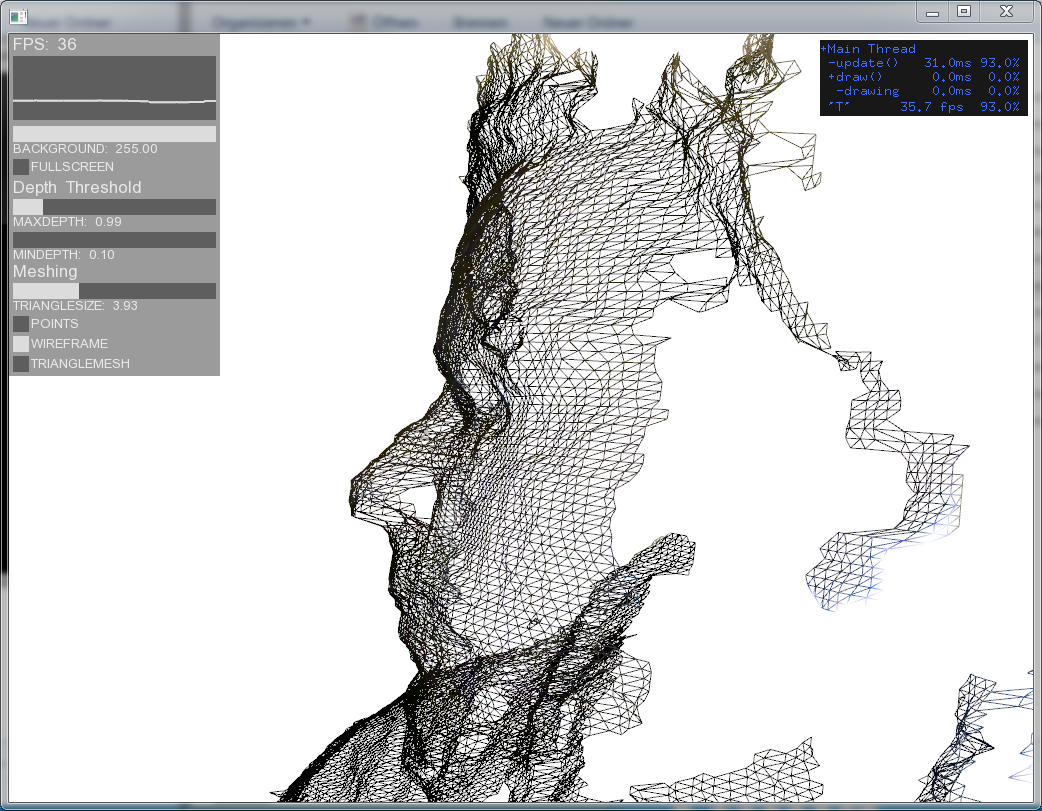
\includegraphics[width=.5\textwidth, keepaspectratio]{img/screen}
		\caption{Screenshot des lokalen User Interface des entwickelten Systems mit Rekonstruktionsergebnis von \textit{Pipeline01} als Wireframedarstellung orthogonal zur Kamerablickrichtung}
		\label{fig:screen}
	\end{center}
\end{figure}
Trotz anfänglicher Schwierigkeiten beim Einrichten der Entwicklungsumgebung ist die Umsetzung des Prototypen für die User-Reconstruction Komponente aus der Theorie in die Praxis soweit gelungen. Es ist eine aus heutiger Sicht flexible, gut verstandene Experimentierumgebung entstanden, welche sich für die weitere Arbeit am Thema Echtzeitrekonstruktion gut eignet. Der vorerst fehlgeschlagenen Versuch den Netzwerkadapter zu implementieren hat noch einmal dazu geführt, das Konzept des Netzwerkadapters zu überdenken. Dadurch wurde ein gemeinsames Verständnis des Netzwerkkommunikationsmodells der Gesamtanwendung vertieft.\\

Für Projekt 2 steht zunächst die Fertigstellung des C++ Netzwerkadapters auf dem Plan. Dies legt die Grundlage für die ersten Tests der Netzwerkkommunikation sowie für die eigentliche Verteilung der Anwendungskomponenten. Der nächste Schritt bei der Entwicklung des User Reconstruction Systems ist die Entwicklung einer Sensor Management Komponente zur Verwaltung mehrerer Sensoren sowie einer Kalibrierungskomponente. Parallel dazu wird eine zweite Entwicklungsumgebung auf der Basis von Windows 8 aufgebaut, um die Einbindung des moderneren Kinect2 Sensors zu ermöglichen.

